\documentclass[12pt]{article}
\author{Lawrence Liu, UID: 405749034}
\usepackage{subcaption}
\usepackage{graphicx}
\usepackage{amsmath}
\usepackage{pdfpages}
\newcommand{\Laplace}{\mathscr{L}}
\setlength{\parskip}{\baselineskip}%
\setlength{\parindent}{0pt}%
\usepackage{xcolor}
\usepackage{listings}
\definecolor{backcolour}{rgb}{0.95,0.95,0.92}
\usepackage{amssymb}
\usepackage{empheq}

\newcommand*\widefbox[1]{\fbox{\hspace{2em}#1\hspace{2em}}}
\lstdefinestyle{mystyle}{
    backgroundcolor=\color{backcolour}}
\lstset{style=mystyle}
\title{Chem 20A Worksheet 3}
\begin{document}
\maketitle
\section*{Problem 1}
\subsection*{(a)}
Cs,Na,Li,Ba,Mg
\subsection*{(b)}
Rb,Ca,Si,N,F 
\section*{Problem 2}
$$Fe^{3+}\to [AR]3d^5$$
$$Cl^{-}\to [Ne]3s^2 3p^6$$
$$Cu\to [Ar]3d^{10}4s^1$$
\section*{Problem 3}
We have that the corresponding energy levels 
would be 
$$E_1=\frac{ch}{\lambda}+\frac{1}{2}m_eV_1^2=4.011
\cdot 10^{-16}J$$
$$E_2=\frac{ch}{\lambda}+\frac{1}{2}m_eV_2^2=4.003\cdot
10^{-16}J$$
$$E_3=\frac{ch}{\lambda}+\frac{1}{2}m_eV_3^2=3.856\cdot 
10^{-16}J$$
$$E_4=\frac{ch}{\lambda}+\frac{1}{2}m_eV_4^2=3.682\cdot
10^{-16}J$$
Which results in the following energy diagram
\begin{center}
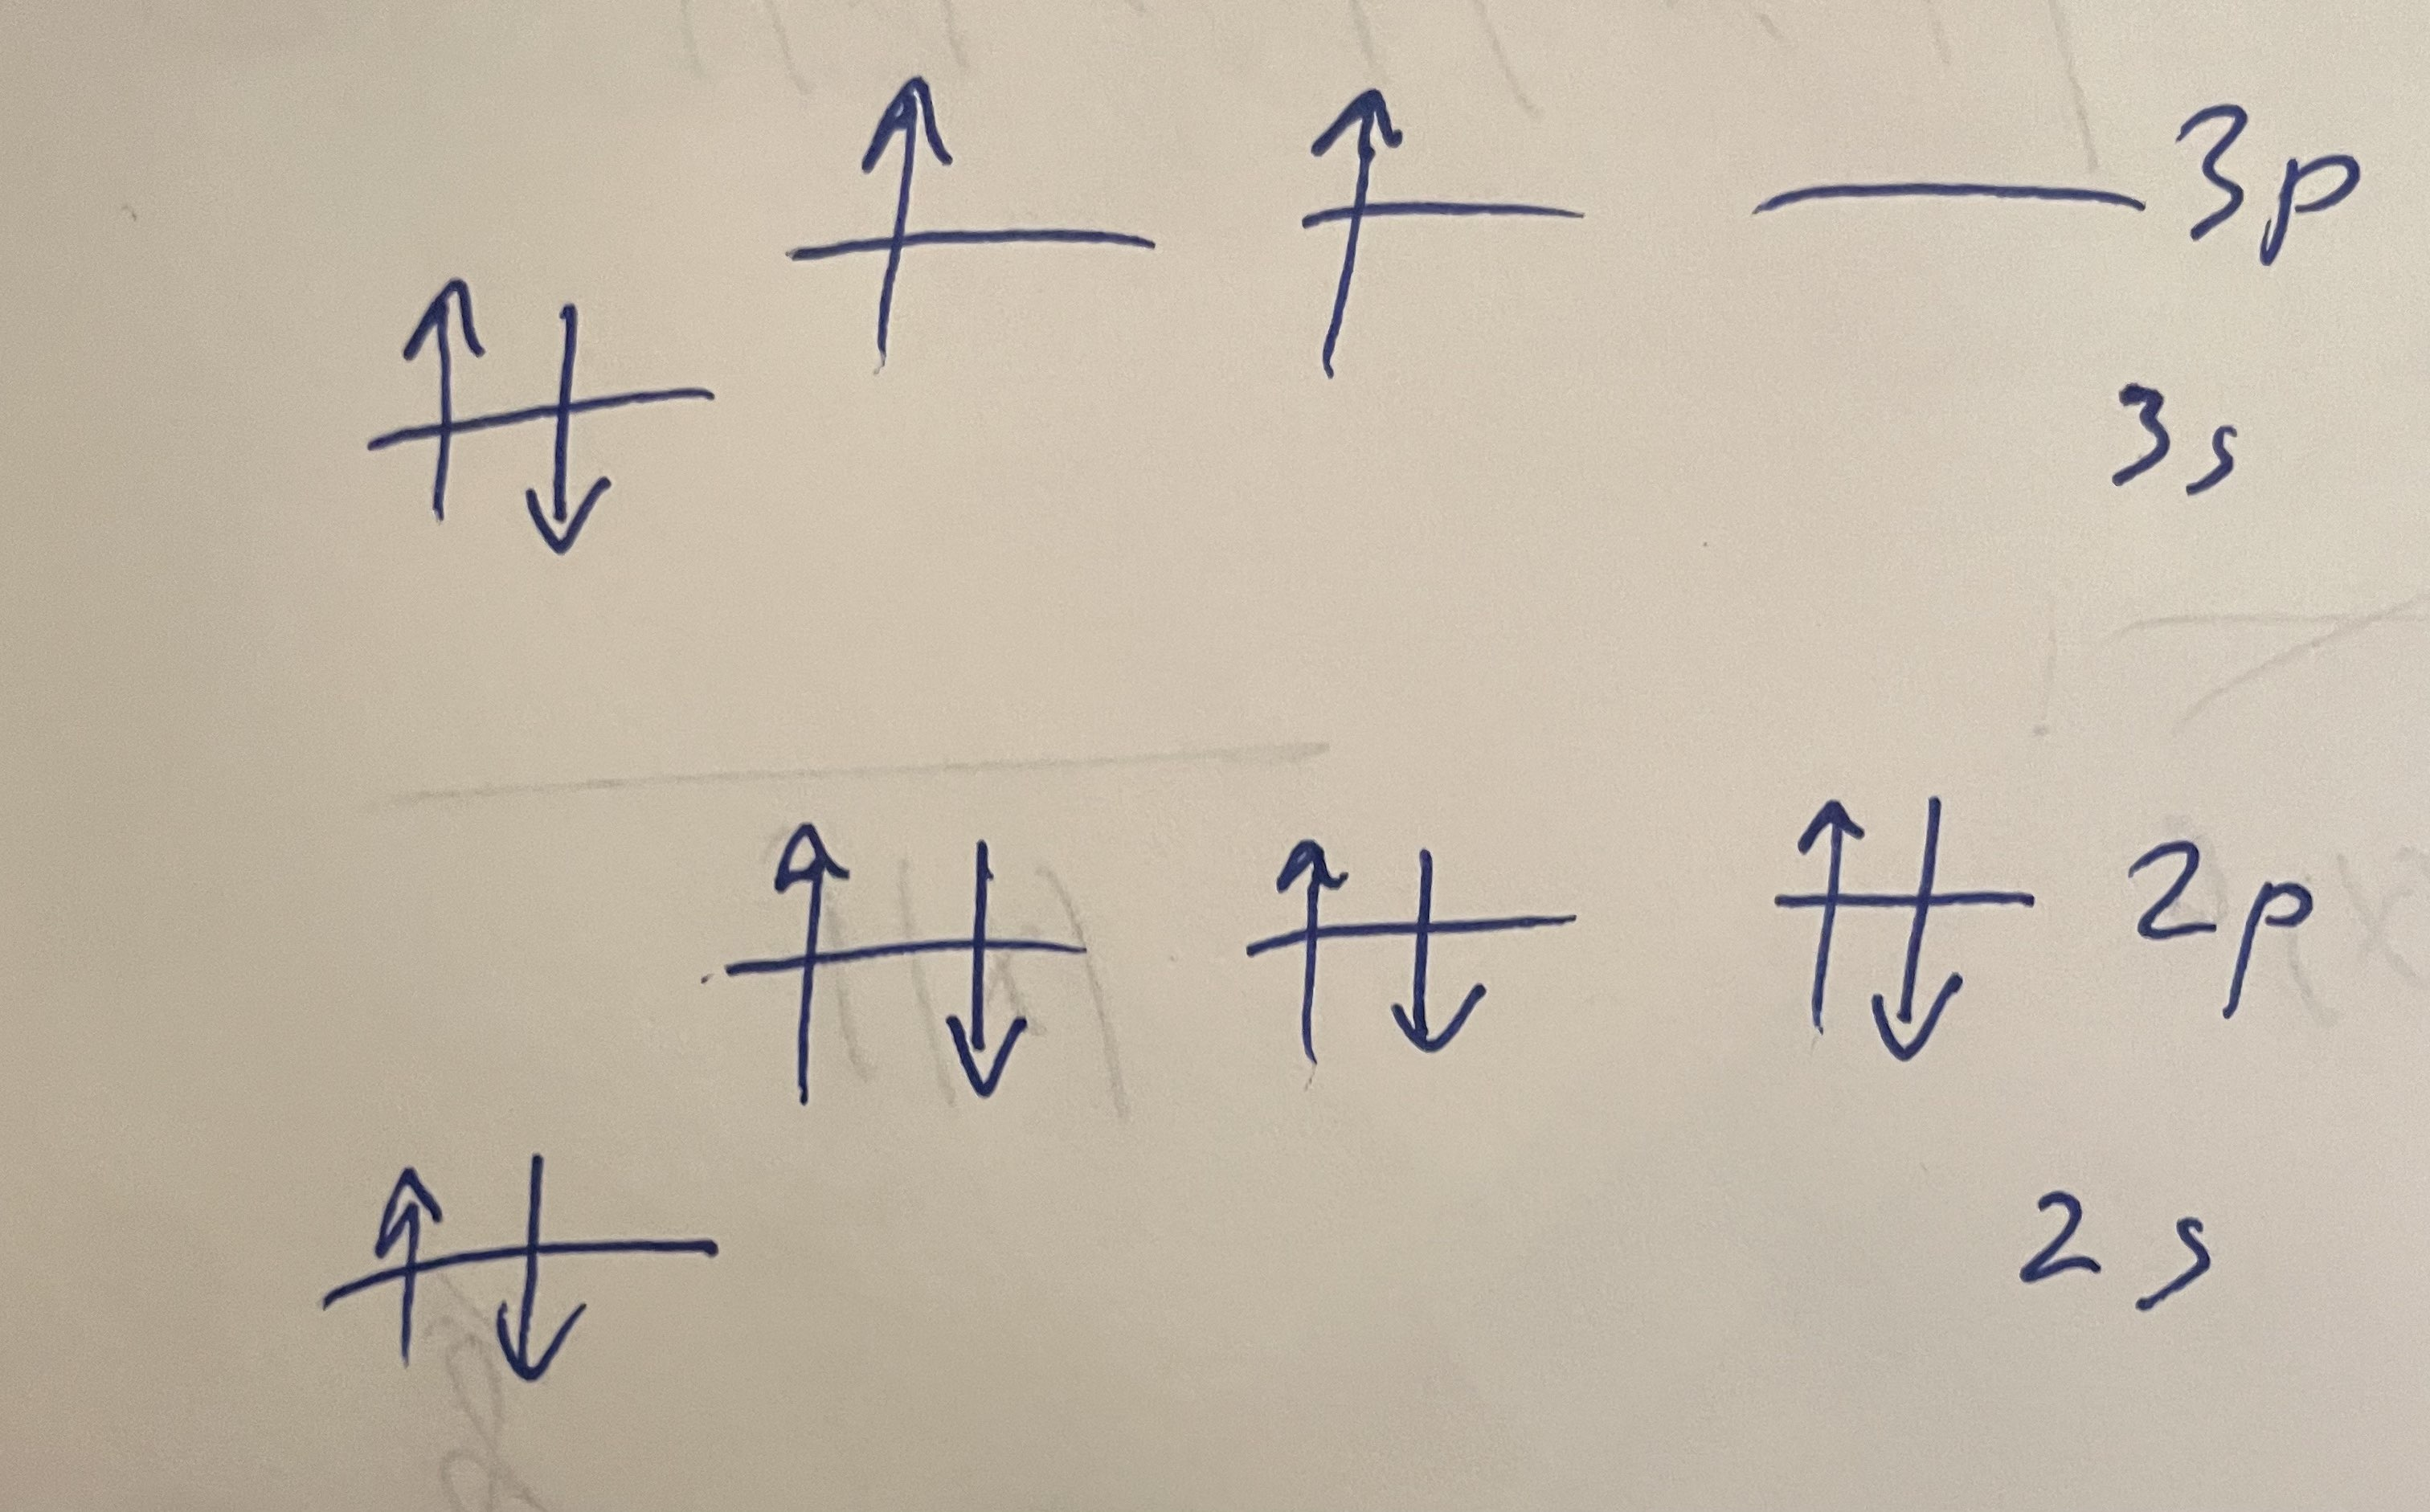
\includegraphics[width=0.5\textwidth]{problem3.png}
\end{center}
\section*{Problem 4}
We have that 
$$E_1=-\frac{8^2}{1}(\text{rydberg})=-8^2\text{rydberg}=-1.395\cdot 10^{-16}J$$
$$E_2=-\frac{(8-3)^2}{2^2}(\text{rydberg})=-\frac{5}{4}\text{rydberg}=-2.724\cdot 10^{-18}J$$
$$E_3=-\frac{(8-6)^2}{2^2}(\text{rydberg})=-\text{rydberg}=-2.179\cdot 10^{-18}J$$
Which results in the following energy level diagram
\begin{center}
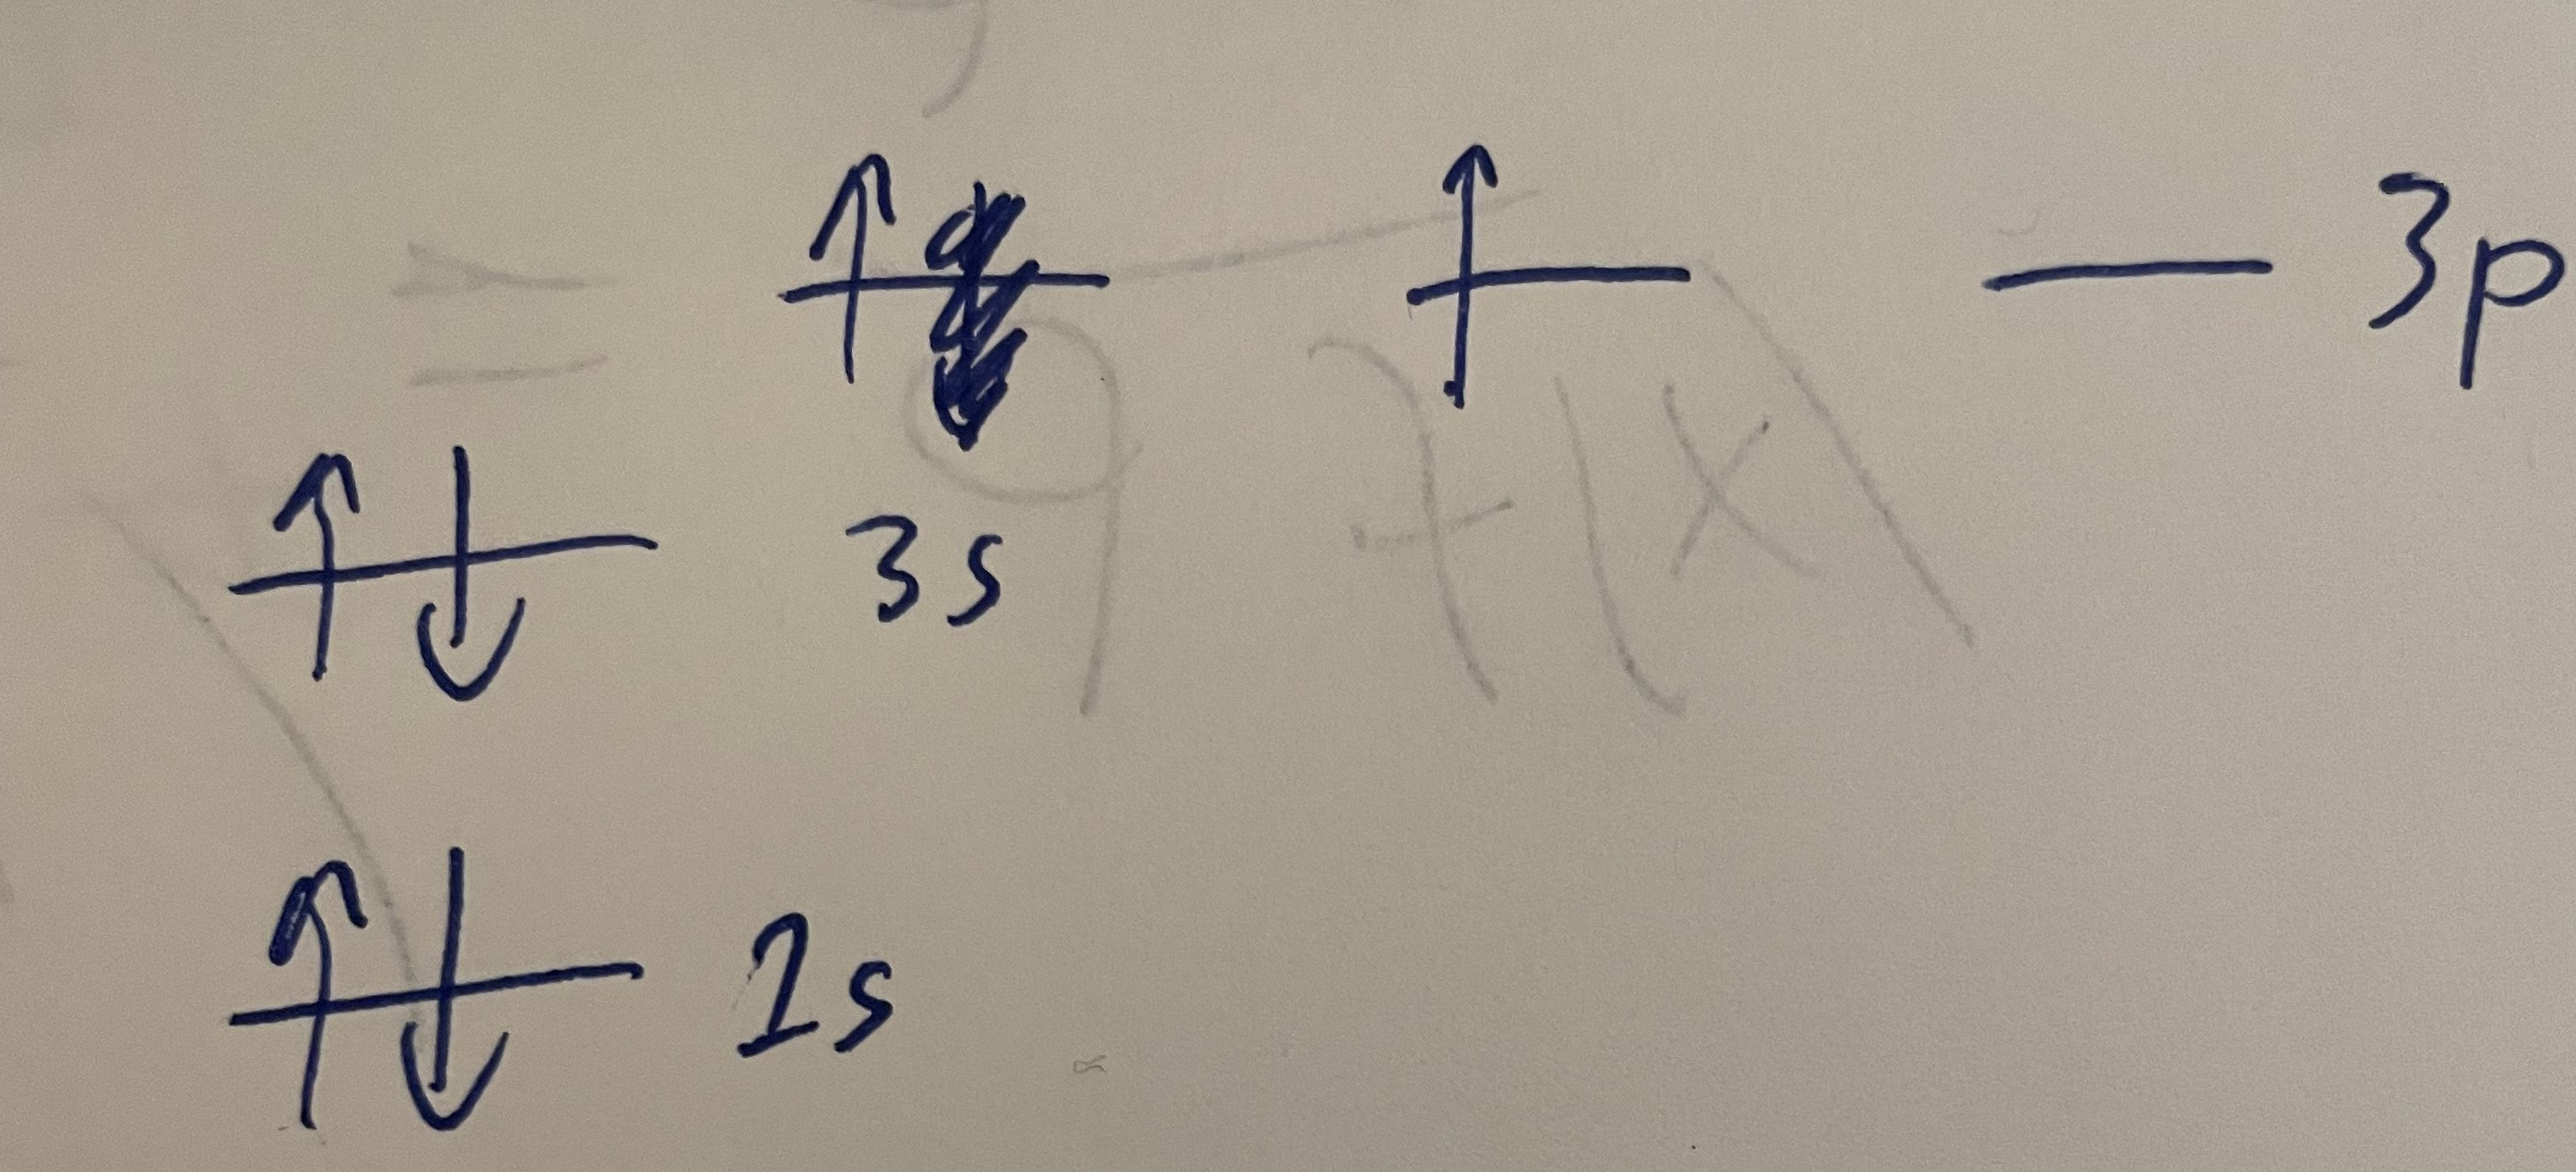
\includegraphics[width=0.5\textwidth]{problem4.png}
\end{center}
\end{document}
